\documentclass[11pt,a4paper]{article}
\usepackage[utf8]{inputenc}
\usepackage[T1]{fontenc}
\usepackage{amsmath, amssymb, amsthm, bm}
\usepackage{geometry}
\usepackage{xcolor}
\usepackage{tcolorbox}
\usepackage{fancyhdr}
\usepackage{tikz}

% Define colors and boxes BEFORE babel to avoid active character conflicts
\definecolor{myblue}{RGB}{0, 80, 150}
\definecolor{mygreen}{RGB}{34, 139, 34}

\newtcolorbox{terimbox}[1]{colback=blue!5!white,colframe=myblue,title=#1}
\newtcolorbox{theoriebox}[1]{colback=green!5!white,colframe=mygreen,title=\textbf{Özet ve Püf Noktalar: #1}}
\newtcolorbox{sonucbox}{colback=white,colframe=gray!50}

% NOTE: babel is intentionally NOT loaded (Turkish babel makes '=' active and breaks TikZ)

\geometry{margin=2.5cm}

\pagestyle{fancy}
\fancyhf{}
\fancyhead[L]{\textbf{Fizik 1 - Devoirs Maison}}
\fancyhead[R]{\textbf{DM1 \& DM2 Çözümleri}}
\fancyfoot[C]{\thepage}

\title{\textcolor{myblue}{\Huge\textbf{Fizik 1 - DM1 \& DM2}}\\[0.3cm]
\Large\textbf{Konu Anlatımlı ve Ayrıntılı Ödev Çözümleri}}
\author{\textbf{Hamza}}
\date{Ekim 2026}

\begin{document}

\maketitle
\tableofcontents
\newpage

%%%%%%%%%%%%%%%%%%%%%%%%%%%%%%%%%%%%%%%%%%%%%%%%%%%%%%%%%%%%%%%%%%%%%%%%%%%%%%%
% PARTIE 1 : DM1
%%%%%%%%%%%%%%%%%%%%%%%%%%%%%%%%%%%%%%%%%%%%%%%%%%%%%%%%%%%%%%%%%%%%%%%%%%%%%%%
\part*{DM 1 : Calcul Vectoriel et Systèmes de Coordonnées}
\addcontentsline{toc}{part}{DM 1 : Calcul Vectoriel et Systèmes de Coordonnées}

\begin{terimbox}{\textbf{Önemli Fransızca Fizik Terimleri (Terminologie Française - DM1)}}
\begin{itemize}
    \item \textbf{Vecteur unitaire:} Birim vektör (uzunluğu 1 olan vektör).
    \item \textbf{Produit scalaire / vectoriel / mixte:} Skaler / Vektörel / Karma çarpım.
    \item \textbf{Repère cartésien / cylindrique:} Kartezyen / Silindirik referans sistemi.
    \item \textbf{Dérivation des vecteurs:} Vektörlerin türevi (zincir kuralına dikkat).
    \item \textbf{Vecteur vitesse:} Hız vektörü (konumun türevi).
    \item \textbf{En déduire:} (Önceki bulgulardan) Yola çıkarak türetmek, çıkarmak.
    \item \textbf{Vérifier:} Doğrulamak, sağlama yapmak.
\end{itemize}
\end{terimbox}

\vspace{0.5cm}

\section*{Exercice 1 : Produits de vecteurs}

\begin{theoriebox}{Vektör Çarpımları ve Bazlar}
\begin{itemize}
    \item \textbf{Norm (Büyüklük):} Bir $\vec{v}$ vektörünün normu $||\vec{v}|| = \sqrt{v_x^2 + v_y^2 + v_z^2}$ formülü ile hesaplanır. Birim vektör ise $\vec{e_v} = \frac{\vec{v}}{||\vec{v}||}$ şeklinde bulunur.
    \item \textbf{Açılar:} İki birim vektörün \textit{skaler çarpımı} aradaki açının kosinüsünü verir ($\vec{e_1} \cdot \vec{e_2} = \cos\theta$). \textit{Vektörel çarpımının} normu ise sinüsünü verir ($||\vec{e_1} \times \vec{e_2}|| = \sin\theta$).
    \item \textbf{Baz Testi:} Üç vektörün bir baz oluşturması için lineer bağımsız olmaları gerekir. Bunun en kolay yolu \textit{determinantın} (karma çarpımın) $0$'dan farklı olduğunu göstermektir.
\end{itemize}
\end{theoriebox}

\subsection*{a) Calcul des normes et des vecteurs unitaires}
Soit les vecteurs $\vec{a}(1,2,2)$, $\vec{b}(2, 2\sqrt{2}, 2)$ et $\vec{c}(0, \sqrt{2}, \sqrt{2})$.
Leurs normes sont :
\begin{align*}
||\vec{a}|| &= \sqrt{1^2 + 2^2 + 2^2} = \sqrt{9} = 3 \\
||\vec{b}|| &= \sqrt{2^2 + (2\sqrt{2})^2 + 2^2} = \sqrt{4 + 8 + 4} = 4 \\
||\vec{c}|| &= \sqrt{0^2 + (\sqrt{2})^2 + (\sqrt{2})^2} = \sqrt{4} = 2
\end{align*}
Les vecteurs unitaires $\vec{e_v} = \frac{\vec{v}}{||\vec{v}||}$ correspondants sont :
\begin{sonucbox}
$\vec{e_a} = \left(\frac{1}{3}, \frac{2}{3}, \frac{2}{3}\right), \quad 
\vec{e_b} = \left(\frac{1}{2}, \frac{\sqrt{2}}{2}, \frac{1}{2}\right), \quad 
\vec{e_c} = \left(0, \frac{\sqrt{2}}{2}, \frac{\sqrt{2}}{2}\right)$
\end{sonucbox}

\subsection*{b) Calcul des cosinus des angles}
Le produit scalaire de deux vecteurs unitaires donne le cosinus de l'angle entre eux :
\begin{align*}
\cos\theta_a &= \vec{e_b} \cdot \vec{e_c} = \left(\frac{1}{2}\right)(0) + \left(\frac{\sqrt{2}}{2}\right)\left(\frac{\sqrt{2}}{2}\right) + \left(\frac{1}{2}\right)\left(\frac{\sqrt{2}}{2}\right) = \frac{2+\sqrt{2}}{4} \\
\cos\theta_b &= \vec{e_a} \cdot \vec{e_c} = \left(\frac{1}{3}\right)(0) + \left(\frac{2}{3}\right)\left(\frac{\sqrt{2}}{2}\right) + \left(\frac{2}{3}\right)\left(\frac{\sqrt{2}}{2}\right) = \frac{4\sqrt{2}}{6} = \frac{2\sqrt{2}}{3} \\
\cos\theta_c &= \vec{e_b} \cdot \vec{e_a} = \left(\frac{1}{2}\right)\left(\frac{1}{3}\right) + \left(\frac{\sqrt{2}}{2}\right)\left(\frac{2}{3}\right) + \left(\frac{1}{2}\right)\left(\frac{2}{3}\right) = \frac{1 + 2\sqrt{2} + 2}{6} = \frac{3+2\sqrt{2}}{6}
\end{align*}

\subsection*{c) Calcul des composantes des vecteurs (produits vectoriels)}
\begin{align*}
\vec{u_a} &= \vec{e_b} \times \vec{e_c} = 
\begin{vmatrix} 
\vec{i} & \vec{j} & \vec{k} \\ 
1/2 & \sqrt{2}/2 & 1/2 \\ 
0 & \sqrt{2}/2 & \sqrt{2}/2 
\end{vmatrix} 
= \vec{i}\left(\frac{2}{4} - \frac{\sqrt{2}}{4}\right) - \vec{j}\left(\frac{\sqrt{2}}{4} - 0\right) + \vec{k}\left(\frac{\sqrt{2}}{4} - 0\right) = \left( \frac{2-\sqrt{2}}{4}, -\frac{\sqrt{2}}{4}, \frac{\sqrt{2}}{4} \right) \\
\vec{u_b} &= \vec{e_c} \times \vec{e_a} = 
\begin{vmatrix} 
\vec{i} & \vec{j} & \vec{k} \\ 
0 & \sqrt{2}/2 & \sqrt{2}/2 \\ 
1/3 & 2/3 & 2/3 
\end{vmatrix} 
= \vec{i}\left(\frac{2\sqrt{2}}{6} - \frac{2\sqrt{2}}{6}\right) - \vec{j}\left(0 - \frac{\sqrt{2}}{6}\right) + \vec{k}\left(0 - \frac{\sqrt{2}}{6}\right) = \left( 0, \frac{\sqrt{2}}{6}, -\frac{\sqrt{2}}{6} \right) \\
\vec{u_c} &= \vec{e_a} \times \vec{e_b} = 
\begin{vmatrix} 
\vec{i} & \vec{j} & \vec{k} \\ 
1/3 & 2/3 & 2/3 \\ 
1/2 & \sqrt{2}/2 & 1/2 
\end{vmatrix} 
= \vec{i}\left(\frac{2}{6} - \frac{2\sqrt{2}}{6}\right) - \vec{j}\left(\frac{1}{6} - \frac{2}{6}\right) + \vec{k}\left(\frac{\sqrt{2}}{6} - \frac{2}{6}\right) = \left( \frac{2-2\sqrt{2}}{6}, \frac{1}{6}, \frac{\sqrt{2}-2}{6} \right)
\end{align*}

\subsection*{d) Déduction des sinus et vérification}
Puisque $||\vec{u}|| = ||\vec{e_1} \times \vec{e_2}|| = ||\vec{e_1}|| \cdot ||\vec{e_2}|| \cdot \sin\theta = \sin\theta$ :
\begin{align*}
\sin\theta_a &= ||\vec{u_a}|| = \sqrt{\left(\frac{2-\sqrt{2}}{4}\right)^2 + \left(-\frac{\sqrt{2}}{4}\right)^2 + \left(\frac{\sqrt{2}}{4}\right)^2} = \sqrt{\frac{10-4\sqrt{2}}{16}} = \frac{\sqrt{10-4\sqrt{2}}}{4} \\
\sin\theta_b &= ||\vec{u_b}|| = \sqrt{0 + \left(\frac{\sqrt{2}}{6}\right)^2 + \left(-\frac{\sqrt{2}}{6}\right)^2} = \sqrt{\frac{4}{36}} = \frac{1}{3} \\
\sin\theta_c &= ||\vec{u_c}|| = \sqrt{\left(\frac{2-2\sqrt{2}}{6}\right)^2 + \left(\frac{1}{6}\right)^2 + \left(\frac{\sqrt{2}-2}{6}\right)^2} = \frac{\sqrt{19-12\sqrt{2}}}{6}
\end{align*}

\textbf{Vérification à l'aide de la question b) :}
On utilise la relation trigonométrique $\sin\theta = \sqrt{1 - \cos^2\theta}$ :
\begin{itemize}
    \item Pour $\theta_a$ : $\cos\theta_a = \frac{2+\sqrt{2}}{4} \implies \cos^2\theta_a = \frac{6+4\sqrt{2}}{16}$. Donc $\sin\theta_a = \sqrt{1 - \frac{6+4\sqrt{2}}{16}} = \frac{\sqrt{10-4\sqrt{2}}}{4}$. (Vérifié)
    \item Pour $\theta_b$ : $\cos\theta_b = \frac{2\sqrt{2}}{3} \implies \cos^2\theta_b = \frac{8}{9}$. Donc $\sin\theta_b = \sqrt{1 - \frac{8}{9}} = \frac{1}{3}$. (Vérifié)
    \item Pour $\theta_c$ : $\cos\theta_c = \frac{3+2\sqrt{2}}{6} \implies \cos^2\theta_c = \frac{17+12\sqrt{2}}{36}$. Donc $\sin\theta_c = \sqrt{1 - \frac{17+12\sqrt{2}}{36}} = \frac{\sqrt{19-12\sqrt{2}}}{6}$. (Vérifié)
\end{itemize}

\subsection*{e) Base et base normée ?}
Pour que les trois vecteurs constituent une base de l'espace, ils doivent être non coplanaires. On vérifie cela en calculant leur produit mixte (le déterminant) :
$$ \det(\vec{u_a}, \vec{u_b}, \vec{u_c}) = 
\begin{vmatrix} 
\frac{2-\sqrt{2}}{4} & -\frac{\sqrt{2}}{4} & \frac{\sqrt{2}}{4} \\[2mm]
0 & \frac{\sqrt{2}}{6} & -\frac{\sqrt{2}}{6} \\[2mm]
\frac{2-2\sqrt{2}}{6} & \frac{1}{6} & \frac{\sqrt{2}-2}{6}
\end{vmatrix} 
$$
En développant par rapport à la première colonne (le terme central est nul car $a_{21}=0$) :
$$ \det = \frac{2-\sqrt{2}}{4}\, M_{11} + \frac{2-2\sqrt{2}}{6}\, M_{31} $$
avec les mineurs :
\begin{align*}
M_{11} &= \left(\frac{\sqrt{2}}{6}\right)\left(\frac{\sqrt{2}-2}{6}\right) - \left(-\frac{\sqrt{2}}{6}\right)\left(\frac{1}{6}\right) = \frac{2-2\sqrt{2}}{36} + \frac{\sqrt{2}}{36} = \frac{2-\sqrt{2}}{36} \\
M_{31} &= \left(-\frac{\sqrt{2}}{4}\right)\left(-\frac{\sqrt{2}}{6}\right) - \left(\frac{\sqrt{2}}{4}\right)\left(\frac{\sqrt{2}}{6}\right) = \frac{2}{24} - \frac{2}{24} = 0
\end{align*}
Donc :
$$ \det = \frac{2-\sqrt{2}}{4} \cdot \frac{2-\sqrt{2}}{36} = \frac{(2-\sqrt{2})^2}{144} = \frac{6-4\sqrt{2}}{144} \neq 0 $$
Puisque le déterminant est non nul, les vecteurs $\vec{u_a}, \vec{u_b}, \vec{u_c}$ \textbf{constituent bien une base}. 
Cependant, pour qu'une base soit normée, il faut que la norme de chaque vecteur soit égale à $1$. Or, d'après la question précédente, $||\vec{u_b}|| = \frac{1}{3} \neq 1$. Cette base \textbf{n'est donc pas normée}.

\newpage

\section*{Exercice 2 : Dérivation des vecteurs unitaires}

\begin{theoriebox}{Vektörlerin Türevi ve Dönen Referans Sistemleri}
\begin{itemize}
    \item \textbf{Zincir Kuralı:} Zamana ($t$) göre türev alırken, açının ($\varphi$) da zamanla değiştiğini hesaba katmalıyız: $\frac{d}{dt} = \frac{d\varphi}{dt} \frac{d}{d\varphi} = \dot{\varphi} \frac{d}{d\varphi}$
    \item \textbf{Kendine Diklik:} Her birim vektörün uzunluğu sabit ($1$) olduğundan, kendi türevi daima kendisine \textit{diktir}. 
    \item \textbf{Bağıl Türev:} Dönen silindirik sistemdeki ($R_{cyl}$) bir gözlemci, kendi eksenlerini ($\vec{e_\rho}, \vec{e_\varphi}$) dönmüyor olarak görür. Bu yüzden o referansta bu vektörlerin türevi $0$'dır.
\end{itemize}
\end{theoriebox}

\subsection*{a) Calcul des dérivées en projection dans la base cartésienne $B$}
Les vecteurs unitaires polaires s'écrivent dans la base cartésienne fixe $B (\vec{e_x}, \vec{e_y}, \vec{e_z})$ :
\begin{align*}
\vec{e_\rho} &= \cos\varphi \vec{e_x} + \sin\varphi \vec{e_y} \\
\vec{e_\varphi} &= -\sin\varphi \vec{e_x} + \cos\varphi \vec{e_y}
\end{align*}
Puisque les vecteurs $\vec{e_x}$ et $\vec{e_y}$ sont fixes dans le repère $R$, on dérive uniquement les coefficients par rapport à $\varphi$ :
\begin{sonucbox}
$$ \left[\frac{d\vec{e_\rho}}{d\varphi}\right]_R = \frac{d(\cos\varphi)}{d\varphi} \vec{e_x} + \frac{d(\sin\varphi)}{d\varphi} \vec{e_y} = -\sin\varphi \vec{e_x} + \cos\varphi \vec{e_y} $$
$$ \left[\frac{d\vec{e_\varphi}}{d\varphi}\right]_R = \frac{d(-\sin\varphi)}{d\varphi} \vec{e_x} + \frac{d(\cos\varphi)}{d\varphi} \vec{e_y} = -\cos\varphi \vec{e_x} - \sin\varphi \vec{e_y} $$
\end{sonucbox}

\subsection*{b) Expressions de ces dérivées dans la base cylindrique $B_{cyl}$}
Pour déduire les expressions dans la base cylindrique, on compare les résultats de la question (a) avec les définitions de $\vec{e_\rho}$ et $\vec{e_\varphi}$.
Pour la première dérivée, on reconnaît exactement l'expression de $\vec{e_\varphi}$ :
$$ -\sin\varphi \vec{e_x} + \cos\varphi \vec{e_y} = \vec{e_\varphi} $$
Pour la deuxième dérivée, en factorisant par le signe moins, on obtient :
$$ -\cos\varphi \vec{e_x} - \sin\varphi \vec{e_y} = -(\cos\varphi \vec{e_x} + \sin\varphi \vec{e_y}) = -\vec{e_\rho} $$
Ainsi, en projection dans la base $B_{cyl}$, on obtient :
\begin{sonucbox}
$$ \left[\frac{d\vec{e_\rho}}{d\varphi}\right]_R = \vec{e_\varphi} $$
$$ \left[\frac{d\vec{e_\varphi}}{d\varphi}\right]_R = -\vec{e_\rho} $$
\end{sonucbox}

\subsection*{c) Expressions par rapport au temps $t$}
Si $\varphi$ est fonction du temps, on applique la règle de la chaîne à l'aide des résultats de la question précédente :
\begin{sonucbox}
$$ \left[\frac{d\vec{e_\rho}}{dt}\right]_R = \left[\frac{d\vec{e_\rho}}{d\varphi}\right]_R \frac{d\varphi}{dt} = \frac{d\varphi}{dt} \vec{e_\varphi} $$
$$ \left[\frac{d\vec{e_\varphi}}{dt}\right]_R = \left[\frac{d\vec{e_\varphi}}{d\varphi}\right]_R \frac{d\varphi}{dt} = -\frac{d\varphi}{dt} \vec{e_\rho} $$
\end{sonucbox}

\subsection*{d) Propriété générale de la dérivée d'un vecteur unitaire}
\textbf{Démonstration :} Soit $\vec{u}$ un vecteur unitaire, donc son produit scalaire par lui-même est constant : $\vec{u} \cdot \vec{u} = 1$.
En dérivant cette relation par rapport au temps :
$$ \frac{d}{dt} (\vec{u} \cdot \vec{u}) = \frac{d\vec{u}}{dt} \cdot \vec{u} + \vec{u} \cdot \frac{d\vec{u}}{dt} = 2 \left( \vec{u} \cdot \frac{d\vec{u}}{dt} \right) = 0 $$
Le produit scalaire étant nul, la dérivée $\frac{d\vec{u}}{dt}$ est orthogonale à $\vec{u}$. Par conséquent, la dérivée de tout vecteur unitaire n'a aucune composante sur lui-même.

\subsection*{e) Le vecteur rotation $\vec{\Omega}$}
On cherche un vecteur $\vec{\Omega} = \Omega_\rho \vec{e_\rho} + \Omega_\varphi \vec{e_\varphi} + \Omega_z \vec{e_z}$ tel que :
$\left[\frac{d\vec{e_\rho}}{dt}\right]_R = \vec{\Omega} \times \vec{e_\rho}$ \quad et \quad $\left[\frac{d\vec{e_\varphi}}{dt}\right]_R = \vec{\Omega} \times \vec{e_\varphi}$ \quad et \quad $\left[\frac{d\vec{e_z}}{dt}\right]_R = \vec{\Omega} \times \vec{e_z}$.

1. Pour $\vec{e_\rho}$ :
\begin{align*}
\vec{\Omega} \times \vec{e_\rho} &= (\Omega_\rho \vec{e_\rho} + \Omega_\varphi \vec{e_\varphi} + \Omega_z \vec{e_z}) \times \vec{e_\rho} = -\Omega_\varphi \vec{e_z} + \Omega_z \vec{e_\varphi}
\end{align*}
Puisque $\left[\frac{d\vec{e_\rho}}{dt}\right]_R = \frac{d\varphi}{dt} \vec{e_\varphi}$, on obtient : $\Omega_\varphi = 0$ et $\Omega_z = \frac{d\varphi}{dt}$.

2. Pour $\vec{e_\varphi}$ :
\begin{align*}
\vec{\Omega} \times \vec{e_\varphi} &= \left(\Omega_\rho \vec{e_\rho} + \frac{d\varphi}{dt} \vec{e_z}\right) \times \vec{e_\varphi} = \Omega_\rho \vec{e_z} - \frac{d\varphi}{dt} \vec{e_\rho}
\end{align*}
Puisque $\left[\frac{d\vec{e_\varphi}}{dt}\right]_R = -\frac{d\varphi}{dt} \vec{e_\rho}$, on obtient : $\Omega_\rho = 0$.

3. Pour $\vec{e_z}$ (Vérification) :
Le vecteur $\vec{e_z}$ est constant dans $R$, donc sa dérivée est nulle.
$\vec{\Omega} \times \vec{e_z} = \left(\frac{d\varphi}{dt} \vec{e_z}\right) \times \vec{e_z} = \vec{0}$. La condition est bien respectée.

On en déduit que le vecteur rotation est :
\begin{sonucbox}
$$ \vec{\Omega} = \frac{d\varphi}{dt} \vec{e_z} $$
\end{sonucbox}

\subsection*{f) Dérivées dans le repère $R_{cyl}$}
\textbf{Pourquoi $\left[\frac{d\vec{e_\rho}}{dt}\right]_{R_{cyl}} = \vec{0}$ et $\left[\frac{d\vec{e_\varphi}}{dt}\right]_{R_{cyl}} = \vec{0}$ ?} \\
Par définition, la notation $\left[\dots\right]_{R_{cyl}}$ implique qu'on dérive par rapport au repère cylindrique. Dans ce repère, qui tourne avec le point, les vecteurs $\vec{e_\rho}$ et $\vec{e_\varphi}$ sont immobiles (constants). La dérivée d'un vecteur constant par rapport à son propre repère est toujours nulle.

\subsection*{g) Calcul des dérivées de $\vec{e_x}$ et $\vec{e_y}$ par rapport à $R_{cyl}$}
On a $\vec{e_x} = \cos\varphi \vec{e_\rho} - \sin\varphi \vec{e_\varphi}$ et $\vec{e_y} = \sin\varphi \vec{e_\rho} + \cos\varphi \vec{e_\varphi}$.
Dans le repère $R_{cyl}$, $\vec{e_\rho}$ et $\vec{e_\varphi}$ sont constants, seul $\varphi$ varie par rapport au temps :
\begin{align*}
\left[\frac{d\vec{e_x}}{dt}\right]_{R_{cyl}} &= -\frac{d\varphi}{dt}\sin\varphi \vec{e_\rho} - \frac{d\varphi}{dt}\cos\varphi \vec{e_\varphi} \\
\left[\frac{d\vec{e_y}}{dt}\right]_{R_{cyl}} &= \frac{d\varphi}{dt}\cos\varphi \vec{e_\rho} - \frac{d\varphi}{dt}\sin\varphi \vec{e_\varphi}
\end{align*}
Ces résultats constituent les \textbf{projections sur la base cylindrique $B_{cyl}$} :
\begin{sonucbox}
$$ \left[\frac{d\vec{e_x}}{dt}\right]_{R_{cyl}} = -\frac{d\varphi}{dt}\sin\varphi \vec{e_\rho} - \frac{d\varphi}{dt}\cos\varphi \vec{e_\varphi} \quad (\text{sur } B_{cyl}) $$
$$ \left[\frac{d\vec{e_y}}{dt}\right]_{R_{cyl}} = \frac{d\varphi}{dt}\cos\varphi \vec{e_\rho} - \frac{d\varphi}{dt}\sin\varphi \vec{e_\varphi} \quad (\text{sur } B_{cyl}) $$
\end{sonucbox}

Ensuite, on factorise ces expressions pour retrouver les vecteurs $\vec{e_x}$ et $\vec{e_y}$ :
Pour $\vec{e_x}$ : $-\frac{d\varphi}{dt} (\sin\varphi \vec{e_\rho} + \cos\varphi \vec{e_\varphi}) = -\frac{d\varphi}{dt} \vec{e_y}$ \\
Pour $\vec{e_y}$ : $\frac{d\varphi}{dt} (\cos\varphi \vec{e_\rho} - \sin\varphi \vec{e_\varphi}) = \frac{d\varphi}{dt} \vec{e_x}$

Ainsi, on obtient les \textbf{projections sur la base cartésienne $B$} :
\begin{sonucbox}
$$ \left[\frac{d\vec{e_x}}{dt}\right]_{R_{cyl}} = -\frac{d\varphi}{dt} \vec{e_y} \quad (\text{sur } B) $$
$$ \left[\frac{d\vec{e_y}}{dt}\right]_{R_{cyl}} = \frac{d\varphi}{dt} \vec{e_x} \quad (\text{sur } B) $$
\end{sonucbox}

\newpage

\section*{Exercice 3 : Vecteur vitesse}

\begin{theoriebox}{Hız Vektörü (Vecteur vitesse)}
\begin{itemize}
    \item Hız, konum vektörünün ($\vec{OP}$) referans sistemine göre zamana göre türevidir.
    \item Eğer bileşenleri tek tek türevliyorsak, \textit{çarpımın türevi} kuralını çok dikkatli uygulamalıyız (hem $\rho$ ve $\varphi$ değişkenlerinin, hem de $\vec{e_\rho}$ vektörünün türevleri alınmalıdır).
\end{itemize}
\end{theoriebox}

\subsection*{a) Expression en coordonnées cartésiennes}
Le vecteur position s'écrit $\vec{OP} = x \vec{e_x} + y \vec{e_y} + z \vec{e_z}$.
Dans le repère $R$, la base $B (\vec{e_x}, \vec{e_y}, \vec{e_z})$ est fixe :
\begin{sonucbox}
$$ \left[\frac{d\vec{OP}}{dt}\right]_R = \frac{dx}{dt} \vec{e_x} + \frac{dy}{dt} \vec{e_y} + \frac{dz}{dt} \vec{e_z} $$
\end{sonucbox}

\subsection*{b) Expression dans $B_{cyl}$ à partir de l'expression cartésienne}
Les relations de passage sont :
$x = \rho \cos\varphi \implies \frac{dx}{dt} = \frac{d\rho}{dt} \cos\varphi - \rho \frac{d\varphi}{dt} \sin\varphi$ \\
$y = \rho \sin\varphi \implies \frac{dy}{dt} = \frac{d\rho}{dt} \sin\varphi + \rho \frac{d\varphi}{dt} \cos\varphi$

En injectant ces expressions et sachant que $\vec{e_x} = \cos\varphi \vec{e_\rho} - \sin\varphi \vec{e_\varphi}$ et $\vec{e_y} = \sin\varphi \vec{e_\rho} + \cos\varphi \vec{e_\varphi}$ :
\begin{align*}
\left[\frac{d\vec{OP}}{dt}\right]_R &= \left(\frac{d\rho}{dt} \cos\varphi - \rho \frac{d\varphi}{dt} \sin\varphi\right)(\cos\varphi \vec{e_\rho} - \sin\varphi \vec{e_\varphi}) \\
&\quad + \left(\frac{d\rho}{dt} \sin\varphi + \rho \frac{d\varphi}{dt} \cos\varphi\right)(\sin\varphi \vec{e_\rho} + \cos\varphi \vec{e_\varphi}) + \frac{dz}{dt} \vec{e_z}
\end{align*}
On développe et on regroupe les termes suivant $\vec{e_\rho}$ et $\vec{e_\varphi}$ :
\textbf{Termes selon $\vec{e_\rho}$ :}
$$ \frac{d\rho}{dt} \cos^2\varphi - \rho \frac{d\varphi}{dt} \sin\varphi \cos\varphi + \frac{d\rho}{dt} \sin^2\varphi + \rho \frac{d\varphi}{dt} \cos\varphi \sin\varphi = \frac{d\rho}{dt}(\cos^2\varphi + \sin^2\varphi) = \frac{d\rho}{dt} $$
\textbf{Termes selon $\vec{e_\varphi}$ :}
$$ -\frac{d\rho}{dt} \cos\varphi \sin\varphi + \rho \frac{d\varphi}{dt} \sin^2\varphi + \frac{d\rho}{dt} \sin\varphi \cos\varphi + \rho \frac{d\varphi}{dt} \cos^2\varphi = \rho \frac{d\varphi}{dt}(\sin^2\varphi + \cos^2\varphi) = \rho \frac{d\varphi}{dt} $$
Finalement :
\begin{sonucbox}
$$ \left[\frac{d\vec{OP}}{dt}\right]_R = \frac{d\rho}{dt} \vec{e_\rho} + \rho \frac{d\varphi}{dt} \vec{e_\varphi} + \frac{dz}{dt} \vec{e_z} $$
\end{sonucbox}

\subsection*{c) Résultat direct depuis $B_{cyl}$}
Le vecteur position s'écrit directement $\vec{OP} = \rho \vec{e_\rho} + z \vec{e_z}$.
En dérivant par rapport au temps dans le repère $R$ :
$$ \left[\frac{d\vec{OP}}{dt}\right]_R = \frac{d\rho}{dt} \vec{e_\rho} + \rho \left[\frac{d\vec{e_\rho}}{dt}\right]_R + \frac{dz}{dt} \vec{e_z} $$
D'après la question 2.c, on sait que $\left[\frac{d\vec{e_\rho}}{dt}\right]_R = \frac{d\varphi}{dt} \vec{e_\varphi}$. Donc :
$$ \left[\frac{d\vec{OP}}{dt}\right]_R = \frac{d\rho}{dt} \vec{e_\rho} + \rho \frac{d\varphi}{dt} \vec{e_\varphi} + \frac{dz}{dt} \vec{e_z} $$
Ce qui est beaucoup plus rapide et direct.

\subsection*{d) Calcul de la vitesse dans le repère $R_{cyl}$}
Si l'on calcule la dérivée de $\vec{OP}$ par rapport au repère cylindrique $R_{cyl}$ :
Les vecteurs unitaires $\vec{e_\rho}$ et $\vec{e_z}$ sont fixes par rapport à ce repère. Ainsi :
\begin{sonucbox}
$$ \left[\frac{d\vec{OP}}{dt}\right]_{R_{cyl}} = \frac{d\rho}{dt} \vec{e_\rho} + \frac{dz}{dt} \vec{e_z} $$
\end{sonucbox}
Le terme angulaire a disparu, il s'agit de la vitesse relative pour un observateur lié au repère tournant.

\newpage

%%%%%%%%%%%%%%%%%%%%%%%%%%%%%%%%%%%%%%%%%%%%%%%%%%%%%%%%%%%%%%%%%%%%%%%%%%%%%%%
% PARTIE 2 : DM2
%%%%%%%%%%%%%%%%%%%%%%%%%%%%%%%%%%%%%%%%%%%%%%%%%%%%%%%%%%%%%%%%%%%%%%%%%%%%%%%
\part*{DM 2 : Cinématique du Point}
\addcontentsline{toc}{part}{DM 2 : Cinématique du Point}

\begin{terimbox}{\textbf{Önemli Fransızca Fizik Terimleri (Terminologie Française - DM2)}}
\begin{itemize}
    \item \textbf{Support de la trajectoire :} Yörünge eğrisi (zaman $t$ parametresini yok ederek elde edilen $y(x)$ veya $x(y)$ kartezyen bağıntısı).
    \item \textbf{Vecteur vitesse $\vec{v_{P/R}}$ :} Hız vektörü ($\vec{v} = \frac{d\vec{OP}}{dt}$), daima yörüngeye teğettir.
    \item \textbf{Vecteur accélération $\vec{a_{P/R}}$ :} İvme vektörü ($\vec{a} = \frac{d\vec{v}}{dt}$), yörüngenin iç bükeyliğine (eğrilik merkezine) doğru bakar.
    \item \textbf{Base de Frenet $(\vec{T}, \vec{N})$ :} Yörüngeye teğet $\vec{T}$ ve dik $\vec{N}$ (merkeze doğru) eksenlerinden oluşan yerel referans sistemi.
    \item \textbf{Accélération tangentielle $a_t$ :} Hızın büyüklüğünün değişim oranı ($a_t = \frac{d||\vec{v}||}{dt} = \frac{\vec{a}\cdot\vec{v}}{||\vec{v}||}$). Hızın büyüklüğünü artırır veya azaltır.
    \item \textbf{Accélération normale $a_n$ :} Hızın yönünün değişim oranı ($a_n = \frac{v^2}{R_c}$). Daima merkeze yöneliktir ($a_n \ge 0$).
    \item \textbf{Mouvement accéléré / retardé / uniforme :} Hızlanan ($\vec{a}\cdot\vec{v} > 0$ veya $\frac{d||\vec{v}||}{dt} > 0$) / Yavaşlayan ($\vec{a}\cdot\vec{v} < 0$) / Düzgün (sabit hızlı, $\frac{d||\vec{v}||}{dt} = 0$).
    \item \textbf{Coordonnées polaires $(\rho, \varphi)$ :} Düzlemde kutupsal koordinatlar. $v_\rho = \dot{\rho}$, $v_\varphi = \rho\dot{\varphi}$.
\end{itemize}
\end{terimbox}

\vspace{0.5cm}

\section*{Exercice 1 : Étude d'une trajectoire en coordonnées cartésiennes}

\begin{theoriebox}{Kartezyen Kinematik ve Frenet Tabanı}
\begin{itemize}
    \item \textbf{Yörünge Denklemi (Équation de la trajectoire) :} $t$ parametresi yok edilir. $y = bt \implies t = y/b$ ifadesi $x = ct^2$ içine yazılırsa bir parabol denklemi elde edilir.
    \item \textbf{Hız ve İvme :} $x(t)$ ve $y(t)$ ifadelerinin zamana göre sırasıyla birinci ve ikinci türevleri alınır. İvme sabit çıkarsa hareket "düzgün değişen" bir karaktere sahiptir.
    \item \textbf{Frenet Bileşenleri :}
    $$ \vec{a} = a_t \vec{T} + a_n \vec{N} \implies ||\vec{a}||^2 = a_t^2 + a_n^2 \implies a_n = \sqrt{||\vec{a}||^2 - a_t^2} $$
    Ayrıca $\vec{a} = ||\vec{a}||\vec{e_x}$ olduğundan, geometri/trigonometri yardımıyla $a_t = ||\vec{a}||\cos\alpha$ ve $a_n = ||\vec{a}||\sin\alpha$ olarak da doğrudan doğrulanır.
\end{itemize}
\end{theoriebox}

Dans le plan $(xOy)$ d'un repère $R(O, \vec{e_x}, \vec{e_y}, \vec{e_z})$, les coordonnées du point $P$ en fonction du temps sont données par :
$$ x(t) = c t^2 \quad \text{et} \quad y(t) = b t \quad (c > 0, \; b > 0) $$

\subsection*{a) Équation cartésienne du support de la trajectoire et représentation}
Pour obtenir l'équation cartésienne de la trajectoire, on élimine le paramètre temporel $t$ entre $x(t)$ et $y(t)$.
De l'expression de $y(t)$, puisque $b > 0$, on exprime $t$ :
$$ t = \frac{y}{b} $$
On reporte cette expression dans $x(t)$ :
$$ x = c \left(\frac{y}{b}\right)^2 = \frac{c}{b^2} y^2 $$
Ce que l'on peut également écrire sous la forme standard d'une parabole d'axe $(Ox)$ :
\begin{sonucbox}
$$ x = \frac{c}{b^2} y^2 \quad \Longleftrightarrow \quad y^2 = \frac{b^2}{c} x \quad (x \ge 0) $$
\end{sonucbox}
\textbf{Description géométrique :} Il s'agit de l'équation d'une \textbf{parabole} de sommet l'origine $O(0,0)$ et d'axe de symétrie l'axe $(Ox)$. Si l'on considère le temps $t \ge 0$, la trajectoire est la demi-branche supérieure de cette parabole ($y \ge 0$).

\subsection*{b) Vecteurs vitesse et accélération}

\subsubsection*{1- Composantes du vecteur vitesse $\vec{v_{P/R}}$}
Le vecteur vitesse est la dérivée temporelle du vecteur position $\vec{OP} = x(t)\vec{e_x} + y(t)\vec{e_y}$ dans le repère fixe $R$ :
$$ \vec{v_{P/R}} = \left[\frac{d\vec{OP}}{dt}\right]_R = \frac{dx}{dt} \vec{e_x} + \frac{dy}{dt} \vec{e_y} $$
Calculons les dérivées des coordonnées :
\begin{align*}
\frac{dx}{dt} &= \frac{d}{dt}(c t^2) = 2ct \\
\frac{dy}{dt} &= \frac{d}{dt}(bt) = b
\end{align*}
Ainsi, les composantes du vecteur vitesse sont :
\begin{sonucbox}
$$ \vec{v_{P/R}} = 2ct \, \vec{e_x} + b \, \vec{e_y} $$
Soit sous forme de composantes cartésiennes :
$$ \begin{pmatrix} v_x \\ v_y \\ v_z \end{pmatrix} = \begin{pmatrix} 2ct \\ b \\ 0 \end{pmatrix} $$
\end{sonucbox}

\subsubsection*{2- Composantes du vecteur accélération $\vec{a_{P/R}}$ et analyse}
Le vecteur accélération est la dérivée temporelle du vecteur vitesse dans le repère $R$ :
$$ \vec{a_{P/R}} = \left[\frac{d\vec{v_{P/R}}}{dt}\right]_R = \frac{dv_x}{dt} \vec{e_x} + \frac{dv_y}{dt} \vec{e_y} $$
Calculons les dérivées des composantes de la vitesse :
\begin{align*}
\frac{dv_x}{dt} &= \frac{d}{dt}(2ct) = 2c \\
\frac{dv_y}{dt} &= \frac{d}{dt}(b) = 0
\end{align*}
Ainsi :
\begin{sonucbox}
$$ \vec{a_{P/R}} = 2c \, \vec{e_x} $$
Soit sous forme de composantes cartésiennes :
$$ \begin{pmatrix} a_x \\ a_y \\ a_z \end{pmatrix} = \begin{pmatrix} 2c \\ 0 \\ 0 \end{pmatrix} $$
\end{sonucbox}

\textbf{Que peut-on dire de $\vec{a_{P/R}}$ ?}
\begin{itemize}
    \item Le vecteur accélération est \textbf{constant} au cours du temps en norme ($||\vec{a}|| = 2c = \text{cste}$), en direction et en sens.
    \item Il est constamment colinéaire à l'axe $(Ox)$ et orienté dans le sens positif de cet axe (car $c > 0$).
\end{itemize}

\subsubsection*{3- Représentation graphique de la trajectoire, de $\vec{v_{P/R}}$ et de $\vec{a_{P/R}}$}
Sur la figure ci-dessous, la parabole $x = \frac{c}{b^2}y^2$ est représentée. En un point $P(t)$ quelconque (pour $t > 0$) :
\begin{itemize}
    \item Le vecteur vitesse $\vec{v_{P/R}}$ est \textbf{tangent} à la parabole en $P$, dirigé dans le sens du mouvement.
    \item Le vecteur accélération $\vec{a_{P/R}}$ est \textbf{horizontal}, parallèle à $\vec{e_x}$ et orienté vers les $x$ croissants (vers l'intérieur de la concavité de la parabole).
\end{itemize}

\begin{center}
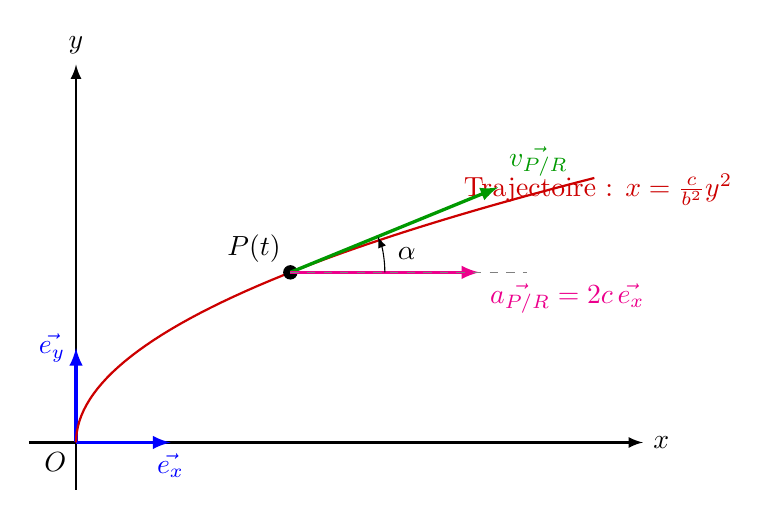
\begin{tikzpicture}[scale=1.2, >=latex]
    % Axes
    \draw[->, thick] (-0.5, 0) -- (6, 0) node[right] {$x$};
    \draw[->, thick] (0, -0.5) -- (0, 4) node[above] {$y$};
    \node[below left] at (0,0) {$O$};
    
    % Unit vectors
    \draw[->, very thick, blue] (0,0) -- (1,0) node[below] {$\vec{e_x}$};
    \draw[->, very thick, blue] (0,0) -- (0,1) node[left] {$\vec{e_y}$};

    % Parabola: x = y^2 * 0.7
    \draw[thick, red!80!black, domain=0:2.8, samples=50] plot ({0.7*\x*\x}, {\x});
    \node[red!80!black, above right] at (4, 2.4) {Trajectoire : $x = \frac{c}{b^2} y^2$};

    % Point P at y = 1.8 -> x = 1.8^2 * 0.7 = 2.268
    \coordinate (P) at (2.268, 1.8);
    \filldraw[black] (P) circle (2pt) node[above left] {$P(t)$};

    % Velocity vector (tangent: slope dx/dy = 2*y*0.7 = 2.52 -> dy/dx = 1/2.52 = 0.396)
    % vx = 2ct, vy = b
    \draw[->, very thick, green!60!black] (P) -- ++(2.2, 0.9) node[above right] {$\vec{v_{P/R}}$};
    
    % Acceleration vector (purely horizontal, along ex)
    \draw[->, very thick, magenta] (P) -- ++(2.0, 0) node[below right] {$\vec{a_{P/R}} = 2c\,\vec{e_x}$};

    % Horizontal reference line from P to show angle alpha
    \draw[dashed, gray] (P) -- ++(2.5, 0);
    \draw[->] (P) ++(1.0, 0) arc (0:22.2:1.0);
    \node at (3.5, 2.0) {$\alpha$};
\end{tikzpicture}
\end{center}

\subsection*{c) Norme de la vitesse, nature du mouvement et composantes de Frenet}

\subsubsection*{1- Calcul de $||\vec{v_{P/R}}||$ et nature du mouvement}
La norme du vecteur vitesse est :
$$ ||\vec{v_{P/R}}|| = \sqrt{v_x^2 + v_y^2} = \sqrt{(2ct)^2 + b^2} $$
\begin{sonucbox}
$$ ||\vec{v_{P/R}}|| = \sqrt{4c^2 t^2 + b^2} $$
\end{sonucbox}

\textbf{Le mouvement est-il accéléré, retardé ou uniforme ?}
Pour déterminer la nature du mouvement, étudions le signe de la dérivée scalaire de la vitesse (ou le produit scalaire $\vec{a}\cdot\vec{v}$) :
\begin{align*}
\frac{d||\vec{v_{P/R}}||}{dt} &= \frac{d}{dt}\left(\sqrt{4c^2 t^2 + b^2}\right) = \frac{8c^2 t}{2\sqrt{4c^2 t^2 + b^2}} = \frac{4c^2 t}{\sqrt{4c^2 t^2 + b^2}}
\end{align*}
De même, par le produit scalaire :
$$ \vec{a_{P/R}} \cdot \vec{v_{P/R}} = (2c)(2ct) + (0)(b) = 4c^2 t $$
Puisque $c > 0$ et pour $t > 0$ :
$$ \vec{a_{P/R}} \cdot \vec{v_{P/R}} > 0 \quad \Longleftrightarrow \quad \frac{d||\vec{v_{P/R}}||}{dt} > 0 $$
La norme de la vitesse est une fonction strictement croissante du temps.
\begin{sonucbox}
Le mouvement est donc \textbf{accéléré} pour $t > 0$ (à l'instant initial $t=0$, l'accélération tangentielle est nulle).
\end{sonucbox}

\subsubsection*{2- Détermination de la composante tangentielle $a_t$ de $\vec{a_{P/R}}$}
Par définition dans le repère de Frenet $(\vec{T}, \vec{N})$, l'accélération tangentielle est donnée par la dérivée de la norme de la vitesse par rapport au temps :
$$ a_t = \frac{d||\vec{v_{P/R}}||}{dt} = \frac{\vec{a_{P/R}} \cdot \vec{v_{P/R}}}{||\vec{v_{P/R}}||} $$
En utilisant les expressions obtenues précédemment :
\begin{sonucbox}
$$ a_t = \frac{4c^2 t}{\sqrt{4c^2 t^2 + b^2}} $$
\end{sonucbox}

\subsubsection*{3- Déduction de la composante normale $a_n$ de $\vec{a_{P/R}}$}
Le repère de Frenet $(\vec{T}, \vec{N})$ forme une base orthonormée. On a donc la relation géométrique :
$$ ||\vec{a_{P/R}}||^2 = a_t^2 + a_n^2 \implies a_n^2 = ||\vec{a_{P/R}}||^2 - a_t^2 $$
Sachant que $||\vec{a_{P/R}}|| = 2c$, d'où $||\vec{a_{P/R}}||^2 = 4c^2$ :
\begin{align*}
a_n^2 &= 4c^2 - \left(\frac{4c^2 t}{\sqrt{4c^2 t^2 + b^2}}\right)^2 \\
&= 4c^2 - \frac{16c^4 t^2}{4c^2 t^2 + b^2} \\
&= \frac{4c^2 (4c^2 t^2 + b^2) - 16c^4 t^2}{4c^2 t^2 + b^2} \\
&= \frac{16c^4 t^2 + 4c^2 b^2 - 16c^4 t^2}{4c^2 t^2 + b^2} = \frac{4c^2 b^2}{4c^2 t^2 + b^2}
\end{align*}
Puisque la composante normale dans la base de Frenet est toujours positive ou nulle ($a_n \ge 0$), et comme $c > 0$ et $b > 0$ :
\begin{sonucbox}
$$ a_n = \sqrt{\frac{4c^2 b^2}{4c^2 t^2 + b^2}} = \frac{2cb}{\sqrt{4c^2 t^2 + b^2}} $$
\end{sonucbox}

\subsection*{d) Angle $\alpha$ et méthode géométrique pour $a_n$}

\subsubsection*{1- Calcul de $\cos\alpha$}
Soit $\alpha$ l'angle orienté entre le vecteur unitaire $\vec{e_x}$ et le vecteur vitesse $\vec{v_{P/R}}$ : $\alpha = (\vec{e_x}, \vec{v_{P/R}})$. \\
Par définition du produit scalaire :
$$ \vec{e_x} \cdot \vec{v_{P/R}} = ||\vec{e_x}|| \cdot ||\vec{v_{P/R}}|| \cos\alpha = 1 \cdot ||\vec{v_{P/R}}|| \cos\alpha $$
D'autre part, en coordonnées cartésiennes :
$$ \vec{e_x} \cdot \vec{v_{P/R}} = v_x = 2ct $$
On en déduit immédiatement :
\begin{sonucbox}
$$ \cos\alpha = \frac{v_x}{||\vec{v_{P/R}}||} = \frac{2ct}{\sqrt{4c^2 t^2 + b^2}} $$
\end{sonucbox}

\subsubsection*{2- Retrouver la composante normale $a_n$ à l'aide de $||\vec{a_{P/R}}||$ et de $\alpha$}
Puisque le vecteur accélération est purement selon $\vec{e_x}$ ($\vec{a_{P/R}} = ||\vec{a_{P/R}}||\vec{e_x} = 2c\vec{e_x}$), l'angle entre $\vec{a_{P/R}}$ et la tangente à la trajectoire (qui porte la vitesse $\vec{v_{P/R}}$ et le vecteur unitaire tangent $\vec{T}$) est précisément $\alpha$.

Le vecteur unitaire $\vec{e_x}$ se projette dans la base de Frenet $(\vec{T}, \vec{N})$ selon :
$$ \vec{e_x} = \cos\alpha \, \vec{T} + \sin\alpha \, \vec{N} $$
Par conséquent, la projection du vecteur accélération $\vec{a_{P/R}}$ donne :
$$ \vec{a_{P/R}} = ||\vec{a_{P/R}}||\cos\alpha \, \vec{T} + ||\vec{a_{P/R}}||\sin\alpha \, \vec{N} $$
On identifie donc la composante normale :
$$ a_n = ||\vec{a_{P/R}}|| \sin\alpha $$
Or, sachant que $\sin^2\alpha = 1 - \cos^2\alpha$ et que $\alpha \in [0, \pi/2]$ :
$$ \sin\alpha = \sqrt{1 - \cos^2\alpha} = \sqrt{1 - \frac{4c^2 t^2}{4c^2 t^2 + b^2}} = \sqrt{\frac{b^2}{4c^2 t^2 + b^2}} = \frac{b}{\sqrt{4c^2 t^2 + b^2}} $$
Comme $||\vec{a_{P/R}}|| = 2c$, on retrouve directement :
\begin{sonucbox}
$$ a_n = 2c \cdot \frac{b}{\sqrt{4c^2 t^2 + b^2}} = \frac{2cb}{\sqrt{4c^2 t^2 + b^2}} $$
\end{sonucbox}
Ce résultat est parfaitement identique à celui obtenu par la relation de Frenet à la question c-3.

\newpage

\section*{Exercice 2 : Mouvement plan circulaire uniforme}

\begin{theoriebox}{Kutupsal Koordinatlarda Dairesel Hareket}
\begin{itemize}
    \item \textbf{Silindirik / Kutupsal Hız Bileşenleri :}
    $$ \vec{v} = \dot{\rho} \vec{e_\rho} + \rho\dot{\varphi} \vec{e_\varphi} $$
    Burada $\varphi = \omega t \implies \dot{\varphi} = \omega$ sabittir.
    \item \textbf{Silindirik / Kutupsal İvme Bileşenleri :}
    $$ a_\rho = \ddot{\rho} - \rho\dot{\varphi}^2, \quad a_\varphi = 2\dot{\rho}\dot{\varphi} + \rho\ddot{\varphi} $$
    \item \textbf{Kartezyen Denkleme Geçiş :}
    Kutupsal denklemin her iki tarafı $\rho$ ile çarpılarak $x = \rho\cos\varphi$, $y = \rho\sin\varphi$ ve $\rho^2 = x^2 + y^2$ özdeşlikleri kullanılır. $x^2 + y^2 - Ax - By = 0$ denklemi tam kareye tamamlanarak $(x-x_C)^2 + (y-y_C)^2 = R^2$ formuna getirilir.
    \item \textbf{Eğrilik Yarıçapı ve İvme Bağıntısı :}
    Düzgün dairesel harekette hız büyüklüğü sabittir ($a_t = 0$). Bu nedenle ivme tamamen normal (merkezcil) ivmedir :
    $$ ||\vec{a}|| = a_n = \frac{v^2}{R} \implies R = \frac{v^2}{||\vec{a}||} $$
\end{itemize}
\end{theoriebox}

Dans le repère $R(O, \vec{e_x}, \vec{e_y})$, un point $P$ a pour coordonnées polaires $\rho$ et $\varphi$ à l'instant $t$ :
$$ \rho(t) = A \cos\varphi + B \sin\varphi \quad \text{avec} \quad \varphi(t) = \omega t $$
où $A, B$ et $\omega$ sont des constantes positives.

\subsection*{a) Composantes cylindriques du vecteur vitesse $\vec{v_{P/R}}$ et nature du mouvement}
Dans le plan $(xOy)$, la base cylindrique (ou polaire) est $(\vec{e_\rho}, \vec{e_\varphi})$. Le vecteur position s'écrit $\vec{OP} = \rho \vec{e_\rho}$. \\
Le vecteur vitesse s'exprime par :
$$ \vec{v_{P/R}} = \left[\frac{d\vec{OP}}{dt}\right]_R = \frac{d\rho}{dt} \vec{e_\rho} + \rho \left[\frac{d\vec{e_\rho}}{dt}\right]_R = \frac{d\rho}{dt} \vec{e_\rho} + \rho \frac{d\varphi}{dt} \vec{e_\varphi} $$
Ses composantes cylindriques sont :
$$ v_\rho = \frac{d\rho}{dt} \quad \text{et} \quad v_\varphi = \rho \frac{d\varphi}{dt} $$
Puisque $\varphi(t) = \omega t$, on a :
$$ \frac{d\varphi}{dt} = \omega $$
Calculons la dérivée de $\rho(t) = A\cos(\omega t) + B\sin(\omega t)$ par rapport au temps :
$$ \frac{d\rho}{dt} = -A\omega \sin(\omega t) + B\omega \cos(\omega t) = \omega (B\cos(\omega t) - A\sin(\omega t)) $$
D'où les composantes :
\begin{align*}
v_\rho &= \omega \bigl(B\cos(\omega t) - A\sin(\omega t)\bigr) \\
v_\varphi &= \rho \omega = \omega \bigl(A\cos(\omega t) + B\sin(\omega t)\bigr)
\end{align*}

\begin{sonucbox}
Les composantes cylindriques du vecteur vitesse sont :
$$ \vec{v_{P/R}} = \omega\bigl(B\cos(\omega t) - A\sin(\omega t)\bigr) \vec{e_\rho} + \omega\bigl(A\cos(\omega t) + B\sin(\omega t)\bigr) \vec{e_\varphi} $$
\end{sonucbox}

\textbf{Nature du mouvement :} \\
Calculons la norme du vecteur vitesse $||\vec{v_{P/R}}||$ :
\begin{align*}
||\vec{v_{P/R}}||^2 &= v_\rho^2 + v_\varphi^2 \\
&= \omega^2 \left[ \bigl(B\cos(\omega t) - A\sin(\omega t)\bigr)^2 + \bigl(A\cos(\omega t) + B\sin(\omega t)\bigr)^2 \right] \\
&= \omega^2 \left[ B^2\cos^2(\omega t) - 2AB\cos(\omega t)\sin(\omega t) + A^2\sin^2(\omega t) \right. \\
&\quad\quad \left. + A^2\cos^2(\omega t) + 2AB\cos(\omega t)\sin(\omega t) + B^2\sin^2(\omega t) \right] \\
&= \omega^2 \left[ (A^2 + B^2)\cos^2(\omega t) + (A^2 + B^2)\sin^2(\omega t) \right] \\
&= \omega^2 (A^2 + B^2) (\cos^2(\omega t) + \sin^2(\omega t)) \\
&= \omega^2 (A^2 + B^2)
\end{align*}
D'où la norme de la vitesse :
\begin{sonucbox}
$$ ||\vec{v_{P/R}}|| = \omega \sqrt{A^2 + B^2} = \text{constante} $$
\end{sonucbox}
Puisque la norme de la vitesse est indépendante du temps ($||\vec{v_{P/R}}|| = \text{cste}$), la vitesse scalaire est constante :
\begin{sonucbox}
Le mouvement est \textbf{uniforme}. \\
(Comme la trajectoire est un cercle d'après la question c, il s'agit d'un \textbf{mouvement circulaire uniforme}).
\end{sonucbox}

\subsection*{b) Composantes cylindriques du vecteur accélération $\vec{a_{P/R}}$}
Dans la base polaire, l'accélération s'écrit $\vec{a_{P/R}} = a_\rho \vec{e_\rho} + a_\varphi \vec{e_\varphi}$, avec :
$$ a_\rho = \frac{d^2\rho}{dt^2} - \rho \left(\frac{d\varphi}{dt}\right)^2 \quad \text{et} \quad a_\varphi = 2\frac{d\rho}{dt}\frac{d\varphi}{dt} + \rho\frac{d^2\varphi}{dt^2} $$
Comme $\varphi = \omega t$, la dérivée seconde angulaire est nulle : $\frac{d^2\varphi}{dt^2} = 0$. \\
Calculons la dérivée seconde $\frac{d^2\rho}{dt^2}$ :
\begin{align*}
\frac{d^2\rho}{dt^2} &= \frac{d}{dt}\left[\omega(-A\sin\omega t + B\cos\omega t)\right] \\
&= \omega(-A\omega\cos\omega t - B\omega\sin\omega t) \\
&= -\omega^2 (A\cos\omega t + B\sin\omega t) = -\omega^2 \rho(t)
\end{align*}
Calculons à présent la composante radiale $a_\rho$ :
\begin{align*}
a_\rho &= -\omega^2 \rho - \rho \omega^2 = -2\omega^2 \rho \\
&= -2\omega^2 (A\cos(\omega t) + B\sin(\omega t))
\end{align*}
Calculons la composante orthoradiale $a_\varphi$ :
\begin{align*}
a_\varphi &= 2 \left(\frac{d\rho}{dt}\right) \omega + 0 \\
&= 2\omega \cdot \omega (-A\sin(\omega t) + B\cos(\omega t)) \\
&= 2\omega^2 (B\cos(\omega t) - A\sin(\omega t))
\end{align*}

\begin{sonucbox}
Les composantes cylindriques du vecteur accélération sont :
\begin{align*}
a_\rho &= -2\omega^2 (A\cos(\omega t) + B\sin(\omega t)) = -2\omega^2 \rho \\
a_\varphi &= 2\omega^2 (B\cos(\omega t) - A\sin(\omega t))
\end{align*}
\end{sonucbox}

Remarquons que la norme de l'accélération est :
\begin{align*}
||\vec{a_{P/R}}||^2 &= a_\rho^2 + a_\varphi^2 = 4\omega^4 (A\cos\omega t + B\sin\omega t)^2 + 4\omega^4 (B\cos\omega t - A\sin\omega t)^2 \\
&= 4\omega^4 (A^2 + B^2)
\end{align*}
Ce qui donne une norme constante :
$$ ||\vec{a_{P/R}}|| = 2\omega^2 \sqrt{A^2 + B^2} = \text{constante} $$

\subsection*{c) Équation cartésienne de la trajectoire et nature circulaire}
Les relations de passage entre coordonnées cartésiennes et coordonnées polaires sont :
$$ x = \rho \cos\varphi, \quad y = \rho \sin\varphi \quad \text{et} \quad \rho^2 = x^2 + y^2 $$
Partons de l'expression de la coordonnée radiale :
$$ \rho = A \cos\varphi + B \sin\varphi $$
Multiplions les deux membres de cette équation par $\rho$ :
$$ \rho^2 = A (\rho \cos\varphi) + B (\rho \sin\varphi) $$
En substituant $x$, $y$ et $\rho^2$ :
$$ x^2 + y^2 = Ax + By $$
Soit :
$$ x^2 - Ax + y^2 - By = 0 $$
Mettons cette équation sous forme canonique :
\begin{align*}
\left(x - \frac{A}{2}\right)^2 - \left(\frac{A}{2}\right)^2 + \left(y - \frac{B}{2}\right)^2 - \left(\frac{B}{2}\right)^2 &= 0 \\
\left(x - \frac{A}{2}\right)^2 + \left(y - \frac{B}{2}\right)^2 &= \frac{A^2}{4} + \frac{B^2}{4} = \frac{A^2 + B^2}{4}
\end{align*}
En posant $R_{cercle} = \frac{\sqrt{A^2 + B^2}}{2}$, l'équation s'écrit :
\begin{sonucbox}
$$ \left(x - \frac{A}{2}\right)^2 + \left(y - \frac{B}{2}\right)^2 = \left(\frac{\sqrt{A^2 + B^2}}{2}\right)^2 $$
\end{sonucbox}
\textbf{Conclusion :} Cette équation est celle d'un \textbf{cercle} de centre $C\left(\frac{A}{2}, \frac{B}{2}\right)$ et de rayon :
$$ R = \frac{\sqrt{A^2 + B^2}}{2} $$
On remarque que pour $(x, y) = (0, 0)$, l'équation est vérifiée ($0^2 + 0^2 = 0$), ce qui montre que le cercle passe par l'origine $O$ du repère.

\begin{center}
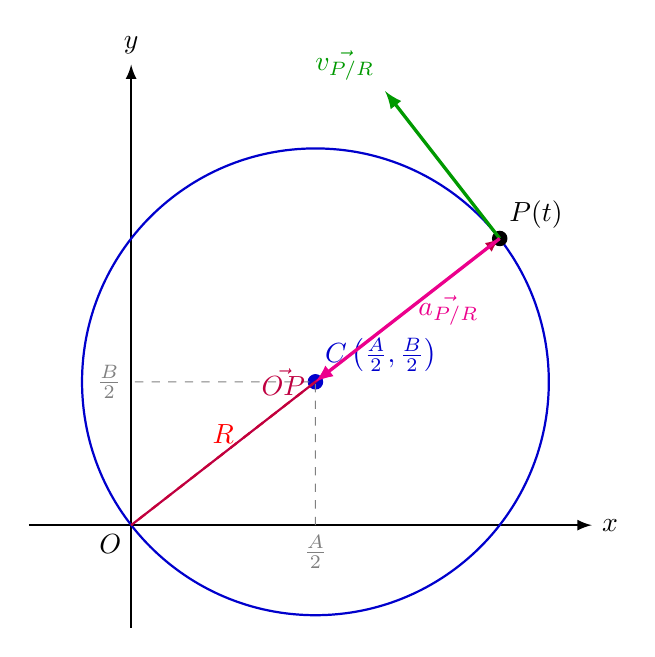
\begin{tikzpicture}[scale=1.3, >=latex]
    % Axes
    \draw[->, thick] (-1, 0) -- (4.5, 0) node[right] {$x$};
    \draw[->, thick] (0, -1) -- (0, 4.5) node[above] {$y$};
    \node[below left] at (0,0) {$O$};

    % Center C (say A=3, B=2 -> C=(1.5, 1))
    \coordinate (C) at (1.8, 1.4);
    
    % Circle passing through O
    \draw[thick, blue!80!black] (C) circle (2.28);
    \filldraw[blue!80!black] (C) circle (2pt) node[above right] {$C\left(\frac{A}{2}, \frac{B}{2}\right)$};
    
    % Center coords dashed
    \draw[dashed, gray] (1.8, 0) node[below] {$\frac{A}{2}$} -- (C) -- (0, 1.4) node[left] {$\frac{B}{2}$};

    % Radius from C to O
    \draw[thick, dashed, red] (C) -- (0,0) node[midway, above] {$R$};
    
    % Point P on circle
    \coordinate (P) at (3.6, 2.8);
    \filldraw[black] (P) circle (2pt) node[above right] {$P(t)$};
    \draw[->, thick, purple] (0,0) -- (P) node[midway, left] {$\vec{OP}$};
    
    % Velocity vector at P (tangent to circle)
    \draw[->, very thick, green!60!black] (P) -- ++(-1.12, 1.44) node[above left] {$\vec{v_{P/R}}$};
    
    % Acceleration vector at P (pointing towards center C)
    \draw[->, very thick, magenta] (P) -- (C) node[midway, right] {$\vec{a_{P/R}}$};
\end{tikzpicture}
\end{center}

\subsection*{d) Déduction du rayon du cercle à partir de l'expression de $||\vec{a_{P/R}}||$}
Pour un mouvement plan quelconque, l'accélération s'exprime dans la base de Frenet par :
$$ \vec{a_{P/R}} = a_t \vec{T} + a_n \vec{N} = \frac{dv}{dt} \vec{T} + \frac{v^2}{R_c} \vec{N} $$
où $v = ||\vec{v_{P/R}}||$ est la vitesse scalaire et $R_c$ est le rayon de courbure de la trajectoire.

Or, d'après la question a), le mouvement est uniforme, ce qui implique que la vitesse scalaire est constante :
$$ v = ||\vec{v_{P/R}}|| = \omega \sqrt{A^2 + B^2} \implies a_t = \frac{dv}{dt} = 0 $$
L'accélération tangentielle étant nulle, l'accélération est \textbf{purement normale} (centripète) :
$$ ||\vec{a_{P/R}}|| = a_n = \frac{v^2}{R_c} $$
Le rayon de courbure $R_c$ (qui correspond ici au rayon $R$ de la trajectoire circulaire) est donc :
$$ R = \frac{v^2}{||\vec{a_{P/R}}||} $$
Remplaçons $v^2$ et $||\vec{a_{P/R}}||$ par leurs expressions :
\begin{align*}
v^2 &= \left(\omega \sqrt{A^2 + B^2}\right)^2 = \omega^2 (A^2 + B^2) \\
||\vec{a_{P/R}}|| &= \sqrt{a_\rho^2 + a_\varphi^2} = 2\omega^2 \sqrt{A^2 + B^2}
\end{align*}
En injectant ces résultats dans l'expression du rayon :
$$ R = \frac{\omega^2 (A^2 + B^2)}{2\omega^2 \sqrt{A^2 + B^2}} = \frac{A^2 + B^2}{2\sqrt{A^2 + B^2}} = \frac{\sqrt{A^2 + B^2}}{2} $$
\begin{sonucbox}
$$ R = \frac{\sqrt{A^2 + B^2}}{2} $$
\end{sonucbox}
On retrouve de manière remarquable et parfaitement cohérente la valeur du rayon obtenue géométriquement à la question c).

\end{document}
